\section{ITree Specification Language}
To write specifications for protocols' rich semantics, I employed ``interaction
tree'' (ITree), a generic data structure for representing interactive programs,
introduced by \textcite{itree}.  ITree enables specifying protocols as monadic
programs that model valid implementations' possible behavior.  The model program
can be interpreted into a tester program, to be discussed in
\autoref{sec:spec-to-test}.

\subsection{Language definition}

\begin{figure}
  \begin{lstlisting}[style=customcoq]
CoInductive itree (E : Type -> Type) (R : Type) :=
| Ret (r : R)
| Vis {X : Type} (e : E X) (k : X -> itree E R)
| Tau (t : itree E R).

Inductive event (E : Type -> Type) : Type :=
| Event : forall X, E X -> X -> event E.

Definition trace E := list (event E)

Inductive is_trace E R
  : itree E R -> trace E -> Prop := ...
  (* straightforward definition omitted *)
 \end{lstlisting}
  \caption{Interaction trees and their traces of events.}
  \label{fig:itrees}
\end{figure}

Figure~\ref{fig:itrees} defines the type \ilc{itree E R}.  The definition is
\textit{coinductive}, so that it can represent potentially infinite sequences of
interactions, as well as divergent behaviors.  The parameter \ilc{E} is a type
of \textit{external interactions}---it defines the interface by which a
computation interacts with its environment.  \ilc{R} is the \textit{result} of
the computation: if the computation halts, it returns a value of type \ilc{R}.

There are three ways to construct an ITree. The \ilc{Ret r} constructor
corresponds to the trivial computation that halts and yields the value
\ilc{r}. The \ilc{Tau t} constructor corresponds to a silent step of
computation, which does something internal that does not produce any visible
effect and then continues as \ilc{t}.  Representing silent steps explicitly with
\ilc{Tau} allows us, for example, to represent diverging computation without
violating Coq's guardedness condition~\cite{coinduction}:

\begin{lstlisting}[style=customcoq]
CoFixpoint spin {E R} : itree E R := Tau spin.
\end{lstlisting}

The final, and most interesting, way to build an ITree is with the \ilc{Vis X e
  k} constructor.  Here, \ilc{e : E X} is a ``visible'' external effect
(including any outputs provided by the computation to its environment) and
\ilc{X} is the type of data that the environment provides in response to the
event.  The constructor also specifies a continuation, \ilc{k}, which produces
the rest of the computation given the response from the environment.  \ilc{Vis}
creates branches in the interaction tree because \ilc{k} can behave differently
for distinct values of type \ilc{X}.

ITree programs can be written in monadic style, where ``\ilc{x <- u;; k(x)}''
substitutes all occurences of ``\ilc{Ret r}'' in \ilc u with ``\ilc{k(r)}''.
Events in an ITree might be sending and receiving messages, or other primitives
actions like making internal choices.  For example, a QAC server can be defined
as:
\begin{lstlisting}[style=customcoq]
  Definition trigger {E R} (e: E R) : itree E R := Vis _ e Ret.
  Variant qacE : Type -> Type :=  (* event type *)
    Recv   : qacE Q               (* receive a query *)
  | Send   : A -> qacE unit       (* send a response *)
  | Choice : qacE C.              (* make a choice   *)
  CoInductive server (sstep: Q -> C -> S -> A * S) (s: S) : itree qacE void :=
    q <- trigger Recv;; c <- trigger Choice;;
    let (a, s') := sstep q c s in trigger (Send a);; server sstep s'.
\end{lstlisting}

\subsection{Interpreting interaction trees}

\begin{figure}
  \lys{Todo: translate to Coq}
  \begin{lstlisting}[style=customcoq,numbers=right,escapechar=\%]
let acc(sum) =
  x := recv(); send(x+sum); acc(x+sum) in
let tee(m) =
  match m with %\label{line:match}%
  | x := recv(); m'(x) =>
    a := recv(); print("IN" ++ a); tee(m'(a))%\label{line:handler1}%
  | send(a); m' =>
    print("OUT" ++ a); send(a); tee(m') %\label{line:handler2}%
  end in
tee(acc(0))
(* ... is equivalent to ... *)
let tee_acc(sum) =
  a := recv(); print("IN" ++ a);
  print("OUT" ++ (a+sum)); send(a+sum);
  tee_acc(a+sum) in
tee_acc(0)
  \end{lstlisting}
  \caption[Interpreting ITree programs.]{Interpretation example.  \ilc{acc} receives a number and returns the
    sum of numbers received so far.  \ilc{tee} prints all the numbers sent and
    received.  Interpreting \ilc{acc} with interpretor \ilc{tee} results in a
    program that's equivalent to \ilc{tee_acc}.}
  \label{fig:logger}
\end{figure}

Interaction tree programs can be destructed into an interaction event followed
by another interaction tree program.  Such structure allows us to {\em
  interpret} one program into another.  \autoref{fig:logger} shows an example of
interpretation: The original \ilc{acc} program sends and receives messages, and
the \ilc{tee} interpretor transforms the \ilc{acc} into another program that
also prints the messages sent and received.

Such interpretation is done by pattern matching on the program's structure in
\autoref{line:match}.  Based on what the original program wants to do next, the
interpretor defines what the result program should do in \autoref{line:handler1}
and \autoref{line:handler2}.  These programs defined in accordance to events are
called {\em handlers}.  By writing different handlers for the events,
interpretors can construct new programs in various ways, as shown in following
subsections.  Further details about interpreting interaction trees are explained
by \textcite{itree}.

\section{Handling External Nondeterminism}
\subsection{Modelling the network}
\label{sec:net-tcp}
The space of network reorderings can be modelled by a {\em network model}, which
is a conceptual program for the ``network wire''.  The wire can be viewed as a
buffer, which can absorb packets and later emit them.  For example, the network
model for concurrent TCP connections is defined as:
\begin{lstlisting}[style=customcoq]
  Variant netE : Type -> Type := (* network event type *)
    Send : packet -> netE unit   (* emit   a packet to   endpoint *)
  | Recv : netE packet           (* absorb a packet from endpoint *)
  | Or   : netE bool.            (* nondeterministic choice       *)
  Definition or (x y: itree netE void) : itree netE void :=
    b <- trigger Or;; if b then x else y.               (* nondeterminstic branch *)
  Fixpoint pick_one (l: list packet) : itree netE (option packet) :=
    if l is p::l' then or (Ret (Some p)) (pick_one l')
    else Ret None.
  Definition oldest_in_each_conn : list packet -> list packet := ...
  CoFixpoint tcp (buffer: list packet) : itree netE void :=  (* TCP network model *)
    let absorb := pkt <- trigger Recv;; tcp (buffer ++ [pkt]) in
    let emit p := trigger (Send p);; tcp (remove pkt buffer)  in
    let pkts := oldest_in_each_conn buffer in
    opkt <- pick_one pkts;;     (* oldest packet in any connection may be emitted *)
    if opkt is Some pkt then emit pkt else absorb.
\end{lstlisting}
The network model introduces an \ilc{Or} event to describe different paths the
system might take.  \ilc{(or x y)} represents a system that is allowed to behave
as either \ilc x or \ilc y.

Notice the \ilc{pick_one} function: Given an empty list, it must return
\ilc{None}, which indicates the network must absorb some packet before emitting
anything.  Given a non-empty list, it might return some element in the list,
which means the network might emit that packet; or it can return \ilc{None},
meaning the network can still absorb packets before emitting any.  This
constructs a network model that reflects TCP, where messages are never lost but
might be indefinitely delayed.

\subsection{Network composition}
\label{sec:net-compose}
The network model is {\em composed} with the server model, yielding a model that
exhibits the ``server delayed by the network'' behavior.  The composition is to
attach the server model as one end on the network model: Assume two message
buffers between the server and the network, \ilc{bi} stores the packets emitted
by the network but not yet consumed by the server, while \ilc{bo} stores the
packets produced by the server but not yet absorbed by the network.  The network
absorbs packets in two ways, either from the servers outgoing buffer \ilc{bo} or
from the clients; Conversely, when the network emits a packet, it either goes to
the client or is appended to the server's incoming buffer
\ilc{bi}:~\footnote{Here for simplicity, the server model uses the same
  \ilc{netE} as the network model.  In practice, the server can be specified
  with a more flexible type interface like \ilc{qacE} in
  \autoref{sec:eval-itree}, provided its events are pairable with the network
  model's \ilc{Send} and \ilc{Recv}.}
\begin{lstlisting}[style=customcoq]
Definition toServer: packet -> bool := ... (* check the packet's destination *)
CoFixpoint compose (srv net: itree netE void) (bi bo: list packet) : itree netE void :=
  match srv, net with
  | Vis vs ks, Vis vn kn =>
    let step_net := (* take a step in the network model *)
      match vn with
      | Recv =>     (* absorb from server whenever possible   *)
        if bo is pkt::bo' then compose srv (kn pkt) bi bo'
                    (* absorb from client if server is silent *)
        else pkt <- trigger Recv;; compose srv (kn pkt) bi bo
      | Send pkt => (* emit packet to its destination *)
        if toServer pkt then       compose srv (kn tt) (bi++[pkt]) bo)
        else  trigger (Send pkt);; compose srv (kn tt)  bi bo
      | Or => b <- trigger Or;; compose srv (kn b) bi bo
      end in
    match vs with
    | Recv =>       (* consume packet from incoming buffer *)
      if bi is pkt::bi' then compose (ks pkt) net bi' bo
      else step_net (* server is starving *)
    | Send pkt =>   (* produce packet to   outgoing buffer *)
      compose (ks tt) net bi (bo++[pkt])
    | Or => b <- trigger Or;; compose (ks b) net bi bo
    end
  | Ret vd, _ | _, Ret vd => match vd in void with end
  end.
\end{lstlisting}
Notice that the composed model schedules the server at a higher priority than
the network model.  Such design is to avoid divergence of the derived tester
program, which was explained in more detail by \textcite{issta21}.

\section{From Specification to Tester}
\label{sec:spec-to-test}

From the server and network models, I derived a tester client that interacts
with servers over the network, and validates the observations against the
protocol specification, as shown in \autoref{fig:framework}.

\begin{figure}
  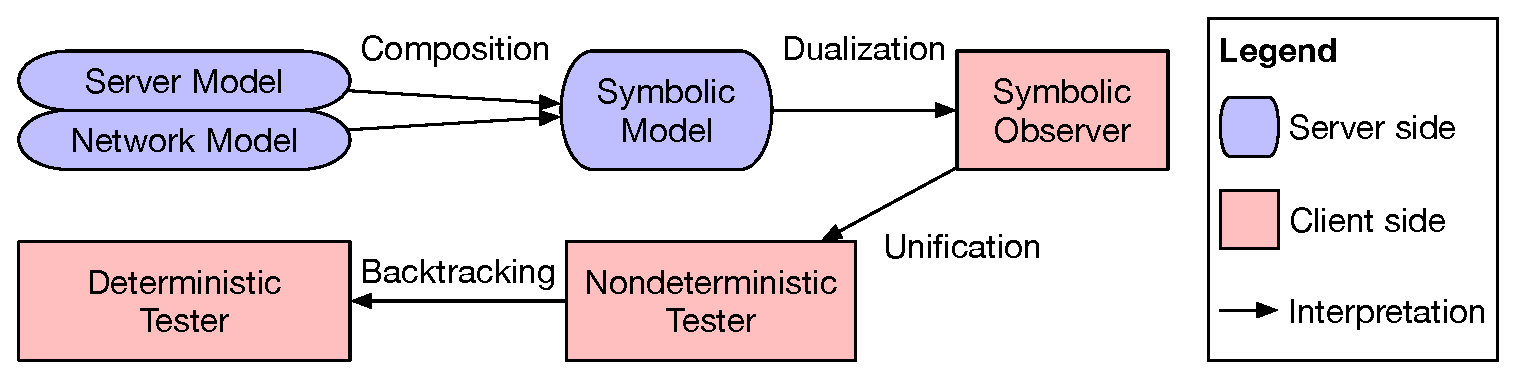
\includegraphics[width=\linewidth]{figures/framework}
  \caption{Deriving tester program from specification}
  \label{fig:framework}
\end{figure}

\subsection{Dualizing ITree model}
To {\em observe} the server's behavior, we have to interpret the specified
server-side events into tester-side events: When the server should send a
certain message, the tester expects to receive the specified message, and
rejects the server upon receiving an unexpected message; when the server should
receive some message, the tester generates a message and sends it to the server,
as shown in \autoref{fig:sym-observe}.

\begin{figure}
  \begin{lstlisting}[style=customcoq]
let observe (server) =
  match server with
  | pkt := recv(); s'(pkt) =>
    p := gen_pkt(); send(p); observe (s'(p))
  | send(pkt); s' =>
    p := recv(); guard(pkt, p); observe (s')
  | IF (x, s1, s2) =>
    (* Allow validating observation with [s1],
     * provided [x] is unifiable with [true];
     * Or, unify [x] with [false],
     * and validate observation with [s2]. *)
    determine(unify(x, true ); observe (s1),
              unify(x, false); observe (s2))
  | r  := _(); s'(r) =>
    r1 := _(); observe (s'(r1))
  end
  \end{lstlisting}
  \caption{Dualizing server model into observer model.  Upon \ilc{recv} events,
    the observer generates a packet and sends it to the server.  For \ilc{send}
    events, the observer receives a packet \ilc{p1}, and fails if it does not
    match the specified \ilc{pkt}.  When the server makes nondeterminstic
    \ilc{IF} branches, the observer \ilc{determine}s between the branches by
    \ilc{unify}ing the branch condition with its conjectured value, and then
    observing the corresponding branch.
    %% Such unification may fail immediately, or add a constraint to the
    %% symbolic variables in \ilc{x}, which instructs future
    %% observations. \bcp{??}
  }
  \label{fig:sym-observe}
\end{figure}

Besides sending and receiving messages, the model also has \ilc{IF} branches
conditioned over symbolic expressions, like that shown in
\autoref{fig:if-match-model}.  Upon nondeterministic branching, the tester needs to
determine which branch was actually taken, by constructing observers for both
branches.  Each branch represents a possible explanation of the server's
behavior.  Upon further interacting with the server, some branches might fail
because its conjecture cannot explain what it has observed.  The tester rejects
the server if all branches have failed, indicating that the server corresponds
to no possible case in the model.
%% \bcp{Very confusing.}

Dualizing the server-side model produces an observer model that performs
interactions to reveal the server's behavior and check its validity.  This model
includes all possible observations from a valid server, and needs to
\ilc{determine} which branch in the server model matches the observed behavior.
The model validates its observations with unification events \ilc{unify} and
\ilc{guard}.  These primitive events are handled by later interpretations: The
\ilc{unify} and \ilc{guard} events in each branch are instantiated into symbolic
evaluation logic that decides whether this branch should fail or not; The
\ilc{determine} events are instantiated into backtracking searches to find if
all branches have failed, which rejects the server.


\subsection{Symbolic Evaluation}

\begin{figure}
  \begin{lstlisting}[style=customcoq,numbers=left,escapechar=\%]
(* unifyS = list variable * list constraint    *)
(* new_var : unifyS -> variable * unifyS        *)
(* assert : exp T * T * unifyS -> option unifyS *)
let unifier (observer, map : mcid -> pcid,
         vars : unifyS) =
  match observer with
  | x := fresh(); o'(x) =>
    let (x1, vars') = new_var(vars) in
    unifier (o'(x1), vars', map)
  | unify(x, v); o' =>
    match assert(x, v, vars) with
    | Some vars' => unifier (o', vars', map)
    | None => failwith "Unexpected payload"
    end
  | guard(p0, p1); o' =>
    match assert(p0, p1, vars) with
    | Some vars' =>
      let mc = p0.source in %\label{line:begin-cid}%
      let pc = p1.source in
      if mc.is_created_by_server
      then match map[mc] with
           | pc => unifier (o', vars', map)
           | unknown =>
             let map' = update(map, mc, pc) in
             unifier (o', vars', map')
           | others =>
             failwith "Unexpected connection"
           end %\label{line:end-cid}%
      else unifier (o', vars', map)
    | None => failwith "Unexpected payload"
    end
  | r  := _(); o'(r) =>
    r1 := _(); unifier (o'(r1), vars, map)
  end\end{lstlisting}
  \caption{Instantiating symbolic events.  The tester maintains a \ilc{unifyS}tate
    which stores the constraints on symbolic variables.  When the
    specification creates a \ilc{fresh} symbol, the tester creates an entry for
    the symbol with no initial constraints.  Upon \ilc{unify} and
    \ilc{guard} events, the tester checks whether the \ilc{assert}ion is
    compatible with the current constraints.  If yes, it updates the constraints
    and move on; otherwise, it raises an error on the current branch.
    %% \sz{We should mention the \ilc{fresh} operation in the main text!}
  }
  \label{fig:unifier}
\end{figure}

In this interpretation phase, we handle nondeterminism at data level by handling
\ilc{fresh} events in the server model, as well as \ilc{unify} and \ilc{guard}
events introduced by dualization.  The interpretor instantiates these events
into symbolic evaluation algorithms.

As shown in \autoref{fig:unifier} (skip
\autoref{line:begin-cid}--\ref{line:end-cid} for now---we'll
explain that part later), the tester checks whether the observed/conjectured
value matches the specification, by maintaining the constraints on the symbolic
variables.  These constraints are initially empty when the variables are
generated by \ilc{fresh} events.  As the test runs into \ilc{unify} and
\ilc{guard} events, it adds constraints \ilc{assert}ing that the observed value
matches the specification, and checks whether the constraints are still
compatible.  Incompatibility among constraints indicates that the server has
exhibited behavior that cannot be explained by the model, implying violation
against the current branch of specification.

\subsection{Handling Incoming Connections}
In addition to generating data internally, the server might exhibit another kind
of nondeterminism related to the outgoing connections it creates.  For example,
when a client uses an HTTP server as proxy, requesting resources from another
server, the proxy server should create a new connection to the target server.
However, as shown in \autoref{fig:proxy-valid-trace}, when the tester receives a
request from an accepted connection, it does not know which client's
request the proxy was forwarding, due to network delays.

Outgoing connections created by the server model are identified by ``model
connection identifiers'' (\ilc{mcid}), and the tester accepts incoming
connections identified by ``physical connection identifiers'' (\ilc{pcid}).  As
shown in \autoref{line:begin-cid}--\ref{line:end-cid} of
\autoref{fig:unifier}, to determine which \ilc{mcid} in the specification does a
runtime \ilc{pcid} corresponds to, the tester maintains a \ilc{map}ping between
the connection identifiers.  Such mapping ensures the tester to check
interactions on an accepted connection against the right connection specified by
the server model.


\subsection{Backtracking}

\begin{figure}
  \begin{lstlisting}[style=customcoq,escapechar=\%]
(* filter : event T * T * list M -> list M *)
(* [filter(e, r, l)] returns a subset in [l],
 * where the model programs' next event is [e]
 * that returns [r]. *)
let backtrack (current, others) =
  match current with
  | determine(t1, t2) =>
    backtrack (t1, t2::others)
  | failwith error => (* current branch failed *) %\label{line:begin-failure}%
    match others with
    | [] => failwith error
    | another::ot' => backtrack (another, ot')
    end %\label{line:end-failure}%
  | send(pkt); t' =>
    let ot' = filter(SEND, pkt, others) in %\label{line:filter-send}%
    send(pkt); backtrack (t', ot')
  | pkt := recv(); t'(pkt) =>
    opkt := maybe_recv();
    match opkt with
    | Some p1 =>
      let ot' = filter(RECV, pkt, others) in %\label{line:filter-recv}%
      backtrack (t'(p1), ot')
    | None =>             (* no packet arrived *)
      match others with
      | [] => backtrack (current, []) (* retry *)
      | another::ot' =>            (* postpone *)
        backtrack (another, ot'++[current])
      end
    end
  end in
backtrack (tester_nondet, [])
  \end{lstlisting}
  \caption{From nondeterministic model to deterministic tester program.  If the
    model makes nondeterministic branches, the tester picks a branch to start
    with, and puts the other branch into a set of other possibilities.  If the
    current branch has failed, the tester looks for other possible branches to
    continue checking.  When the current branch sends a packet, the tester
    filters the set of other possibilities, and only keeps the branches that
    match the current send event.  If the model wants to receive a packet, the
    tester handles both cases whether some packet has arrived or not.}
  \label{fig:backtrack}
\end{figure}

Symbolic evaluation determines whether the observations matches the tester's
conjectures on each branch.  So far, the derived tester
is a nondeterministic program that rejects the server if and only if all
possible branches have raised some error.  To simulate this tester on a
deterministic machine, we execute one branch until it fails.  Upon failure in
the current branch, the simulator switches to another possible branch, until it
exhausts all possibilities and rejects the server, as shown in
\autoref{line:begin-failure}--\ref{line:end-failure} of
\autoref{fig:backtrack}.

When switching from one branch to another, the tester cannot revert its previous
interactions with the server.  Therefore, it must match the server model against
all interactions it has performed, and filter out the mismatching branches, as
shown in \autoref{line:filter-send} and \autoref{line:filter-recv} of
\autoref{fig:backtrack}.
%% , utilizing the lazy evaluation nature of our
%% specification language.\sz{Mention this earlier when introducing Galina?}

We've now derived a tester from the server model.  The specified server runs
forever, and so does the tester (upon no violations observed).  We accept the
server if the tester hasn't rejected it after some large, pre-determined number
of steps of execution.


\iffalse
\section{Specification Languages}

\subsection{Property-based specification with QuickChick}
My first formal specification of \http was written as
QuickChick~\cite{quickchick} properties, which takes a trace of requests, and
determines whether the traces is valid per protocol specification, like that
shown in \autoref{fig:etag-tester}.  The specification implemented a constraint
solving logic by hand, making it hard to scale when the protocol becomes more
complex, as discussed in \autoref{sec:challenges}

\subsection{Model-based specification with ITrees}

From an ITree specification, I conducted ``offline'' testing, which takes a
trace and determines its validity~\cite{cpp19}, and ``online'' testing, where
the specification is derived into a client program that validates the system
under test interactively~\cite{issta21}.

\subsection{Offline testing of swap server}
I started with testing a simple ``swap server''~\cite{cpp19}, specified in
\autoref{fig:linear-spec}.  The specification says that the server can either
accept a connection with a new client (\ilc{obs_connect}) or else receive a
message from a client over some established connection (\ilc{obs_msg_to_server}
\ilc{c}), send back the current stored message (\ilc{obs_msg_from_server}
\ilc{c} \ilc{last_msg}), and then start over with the last received message as
the current state.

To test this swap server, I wrote a client program that interacts with the
server and produces a trace of requests and responses, and a function that
determines whether the trace $t$ is a trace of the linear specification $s$ {\it
  i.e.} whether \ilc{is_trace s t} in \autoref{fig:itrees} holds.

To network nondeterminism, the checker enumerates all possible server-side
message orders that can explain the client-side observations, and checks if any
of them satisifes the protocol specification.
\begin{figure}
\begin{lstlisting}[style=customcoq]
  CoFixpoint linear_spec' (conns : list connection_id)
             (last_msg : bytes) : itree specE unit :=
    or ( (* Accept a new connection. *)
         c <- obs_connect;;
         linear_spec' (c :: conns) last_msg )
       ( (* Exchange a pair of messages on a connection. *)
         c <- choose conns;;
         msg <- obs_msg_to_server c;;
         obs_msg_from_server c last_msg;;
         linear_spec' conns msg ).

  Definition linear_spec := linear_spec' [] zeros.
\end{lstlisting}
\caption[Linear specification of a swap server.]{Linear specification of the
  swap server.  In the \ilc{linear_spec'} loop, the parameter \ilc{conns}
  maintains the list of open connections, while \ilc{last_msg} holds the message
  received from the last client (which will be sent back to the next client).
  The server repeatedly chooses between accepting a new connection or doing a
  receive and then a send on some existing connection picked in the list
  \ilc{conns}.  The linear specification is initialized with an empty set of
  connections and a message filled with zeros.}
\label{fig:linear-spec}
\end{figure}

\subsection{Online testing of HTTP}

Using this automatially derived tester program, I have found violations against
HTTP/1.1 in the latest version of both Apache and Nginx.  More details are
explained in \textcite{issta21}.

\subsection{Key innovation}
To solve the problem of ``determinining whether an observation is explainable by
a nondeterministic program'', I reduced it into a constraint
satisfiability: Although the tester doesn't know the server and network's exact
choices, it can gain some knowledge of these invisible choices by observing the
trace of messages.  If the invisible choices are represented as symbolic
variables, then an observed trace is valid if there exists some value for the
variables that explains this trace, which can be determined by a constraint
solver.

\fi
